\documentclass{beamer}
\usepackage[utf8]{inputenc}

\usetheme{Madrid}
\usecolortheme{default}
\usepackage{amsmath,amssymb,amsfonts,amsthm}
\usepackage{txfonts}
\usepackage{tkz-euclide}
\usepackage{listings}
\usepackage{adjustbox}
\usepackage{array}
\usepackage{tabularx}
\usepackage{gvv}
\usepackage{lmodern}
\usepackage{circuitikz}
\usepackage{tikz}
\usepackage{graphicx}

\setbeamertemplate{page number in head/foot}[totalframenumber]

\lstset{
    language=C,
    basicstyle=\ttfamily\small,
    keywordstyle=\color{blue},
    stringstyle=\color{orange},
    commentstyle=\color{green!60!black},
    numbers=left,
    numberstyle=\tiny\color{gray},
    breaklines=true,
    showstringspaces=false,
}

\title{MatGeo Assignment 1.2.14}
\author{AI25BTECH11008\\Chiruvella Harshith Sharan}
\begin{document}

\frame{\titlepage}

\begin{frame}{Question}
The fourth vertex $D$ of a parallelogram $ABCD$ whose three vertices are 
$A(-2,3)$, $B(6,7)$ and $C(8,3)$ is
\end{frame}

\begin{frame}{Theoretical Solution}
\noindent
We solve this using \textbf{vector algebra}. \\

We are given three vertices of a parallelogram:
$$A(-2,3), \; B(6,7), \; C(8,3).$$
\end{frame}

\begin{frame}{Property}
\textbf{In a parallelogram, opposite sides are parallel and equal.}  

Thus, the fourth vertex is obtained as:
\[
\vec{D} = \vec{A} + \vec{C} - \vec{B}.
\]
\end{frame}

\begin{frame}{Theoretical Solution}
Substitute the given values:  

\[
\vec{D} = \myvec{-2 \\ 3} + \myvec{8 \\ 3} - \myvec{6 \\ 7}
\]

\[
= \myvec{0 \\ -1}
\]

\[
\therefore \; D(0,-1)
\]
\end{frame}

\begin{frame}[fragile]
\frametitle{C-code (Vector Algebra Method)}
\begin{lstlisting}
#include <stdio.h>

int main() {
    // Given vertices
    int x1 , y1 ;  // A
    int x2 , y2 ;  // B
    int x3 , y3 ;  // C
    int x, y;      // D (to be calculated)

    printf("Enter coordinates of A: ");
    scanf("%d %d", &x1, &y1);

    printf("Enter coordinates of B: ");
    scanf("%d %d", &x2, &y2);

    printf("Enter coordinates of C: ");
    scanf("%d %d", &x3, &y3);

    // Using vector algebra property: D = A + C - B
    x = x1 + x3 - x2;
    y = y1 + y3 - y2;

    printf("The fourth vertex D is: (%d, %d)\n", x, y);

    return 0;
}
\end{lstlisting}
\end{frame}

\begin{frame}{Plot}
    \centering
    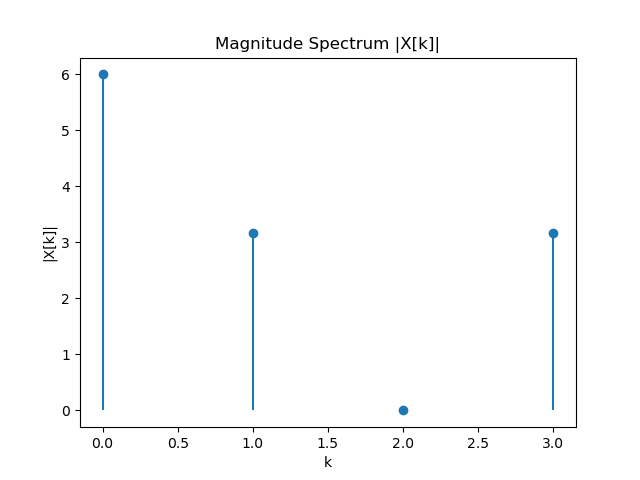
\includegraphics[width=\columnwidth, height=0.8\textheight, keepaspectratio]{figs/fig1.png} 
    \label{Parallelogram ABCD using vector algebra}
\end{frame}

\begin{frame}[fragile]
\frametitle{Python code for plot}
\begin{lstlisting}
import matplotlib.pyplot as plt

# Given points
A = (-2, 3)
B = (6, 7)
C = (8, 3)
D = (0, -1)  # calculated fourth vertex

# Plotting the parallelogram
x_coords = [A[0], B[0], C[0], D[0], A[0]]
y_coords = [A[1], B[1], C[1], D[1], A[1]]

plt.figure(figsize=(6,6))
plt.plot(x_coords, y_coords, 'b-o')

# Plot diagonals
plt.plot([A[0], C[0]], [A[1], C[1]], 'r--', label='Diagonal AC')
plt.plot([B[0], D[0]], [B[1], D[1]], 'g--', label='Diagonal BD')
\end{lstlisting}
\end{frame}

\begin{frame}[fragile]
\frametitle{Python code for plot}
\begin{lstlisting}
# Label points
plt.text(A[0]-0.4, A[1]-0.3, 'A(-2,3)', fontsize=10)
plt.text(B[0]+0.1, B[1], 'B(6,7)', fontsize=10)
plt.text(C[0]+0.1, C[1]-0.3, 'C(8,3)', fontsize=10)
plt.text(D[0]-0.6, D[1]-0.3, 'D(0,-1)', fontsize=10)

# Axes and grid
plt.axhline(0, color='black', linewidth=0.5)
plt.axvline(0, color='black', linewidth=0.5)
plt.grid(True, linestyle='--', alpha=0.5)

# Title and legend
plt.legend()
plt.title("Parallelogram ABCD with diagonals AC and BD")

plt.show()
\end{lstlisting}
\end{frame}

\begin{frame}{Conclusion}
From the figure it is clearly verified that the vector algebra solution matches with the computational solution.
\end{frame}

\end{document}

